\chapter{Тестирование разработанных систем}
\label{ch:chapter5}

В данной главе представлены результаты тестирования двух ключевых компонентов разработанной системы: планировщика упаковки (на базе Timefold Solver) и модуля генерации кода ограничений, построенного на основе нейросетевой модели и взаимодействующего через Docker-контейнеры.

\section{Тестирование работы планировщика}

\subsection{Сравнение качества решений при разном времени планирования}

В рамках эксперимента была проанализирована эффективность работы планировщика на примере производственной заявки от \textbf{25.05.2025}. Была выполнена серия запусков с разным лимитом времени на оптимизацию: 90, 120 и 150 секунд. Для наглядного сравнения на рис.~\ref{fig:quarkus_90sec}, ~\ref{fig:quarkus_120sec}, ~\ref{fig:quarkus_150sec} представлены скриншоты с результатами планирования в интерфейсе Quarkus.

Несмотря на то, что при расчёте за \textbf{90 секунд} значения штрафов по жёстким и средним ограничениям равны нулю (что свидетельствует о корректности с точки зрения допустимости), визуальный анализ показывает наличие существенных недостатков:

\begin{figure}[ht]
 \centering
        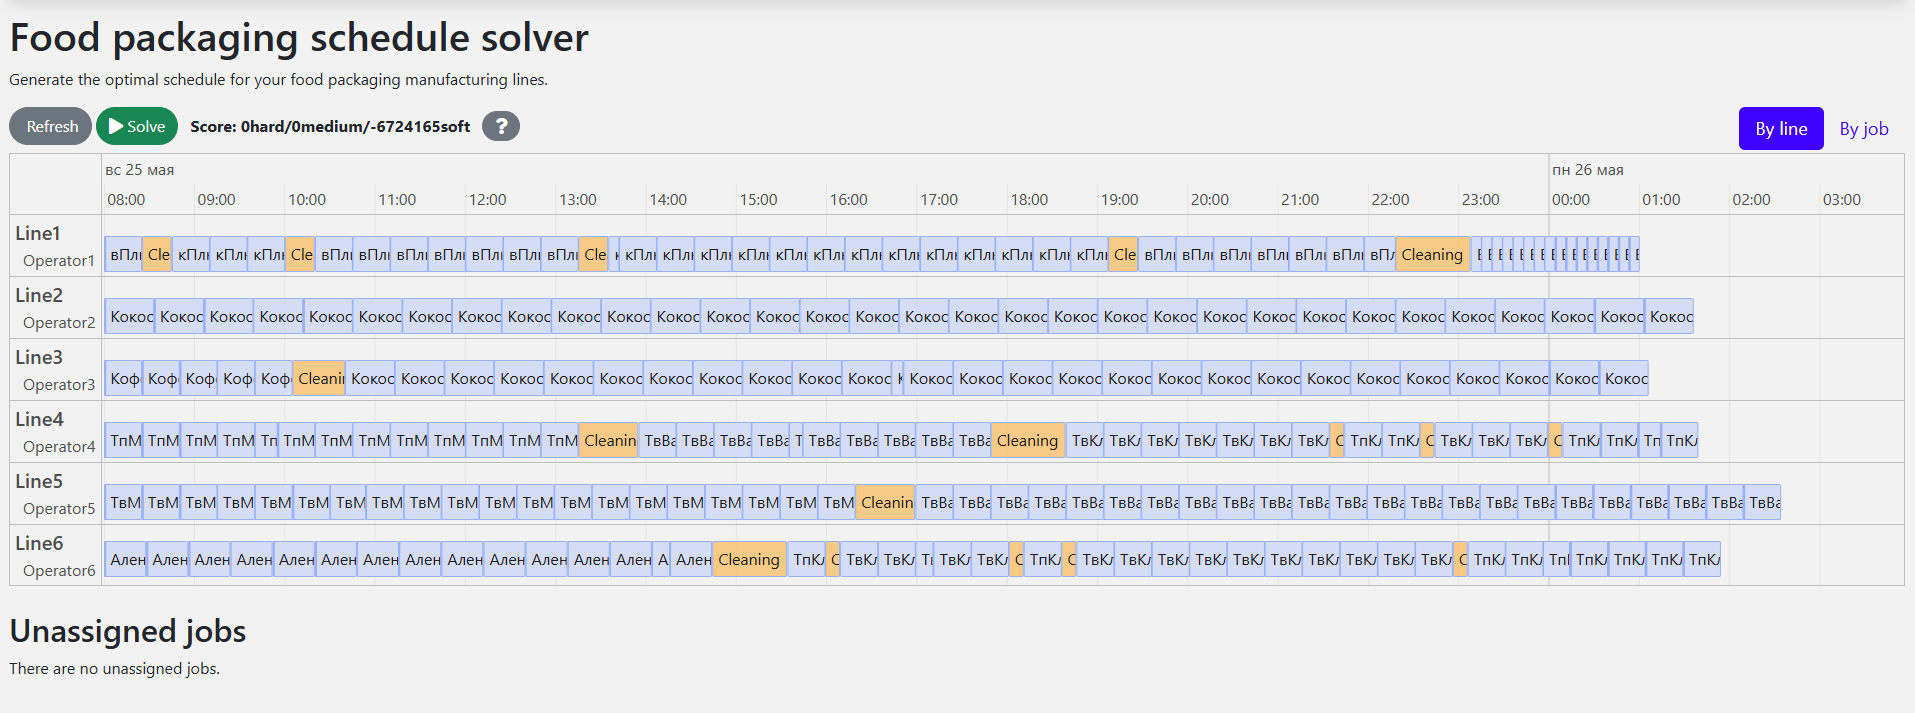
\includegraphics[height = 6 cm, keepaspectratio]{../assets/images/tests/90sec.png}
		\caption{Заявка за 25.05.2025. Время расчета 90 секунд.}
		\label{fig:quarkus_90sec}
\end{figure}

\begin{itemize}
\item одинаковая продукция не идёт подряд на линии, а разбивается другими задачами;
\item возникают лишние фазы санитарной обработки (мойки), которые можно было бы избежать при более компактной упаковке;
\item нарушение логической последовательности заданий внутри одной линии.
\end{itemize}

При увеличении времени до \textbf{120 секунд} ситуация улучшается: количество лишних моек сокращается, продукция начинает группироваться более рационально. Однако и в этом случае сохраняются избыточные переходы между разными типами продукции, что указывает на необходимость более глубокой оптимизации.

\begin{figure}[ht]
 \centering
        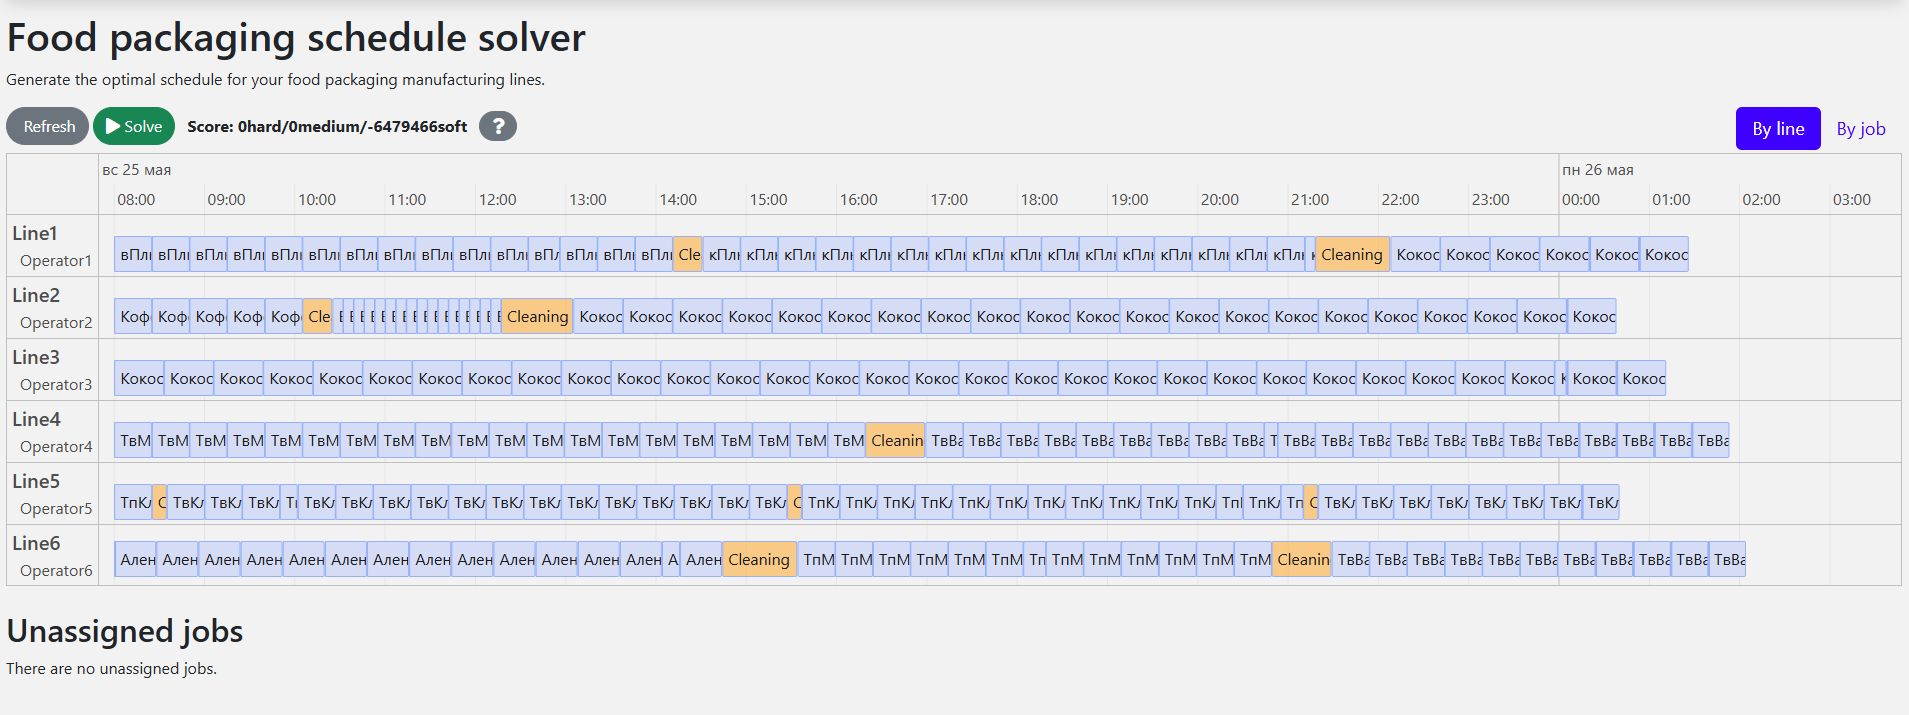
\includegraphics[height = 6 cm, keepaspectratio]{../assets/images/tests/120sec.png}
		\caption{Заявка за 25.05.2025. Время расчета 120 секунд.}
		\label{fig:quarkus_120sec}
\end{figure}

Оптимальное качество решения достигается при расчёте за \textbf{150 секунд}, где:

\begin{itemize}
\item все жёсткие и средние ограничения выполнены;
\item продукция одного типа размещена последовательно;
\item минимизировано количество санитарных обработок;
\item соблюдён приоритет заданий.
\end{itemize}

\begin{figure}[ht]
 \centering
        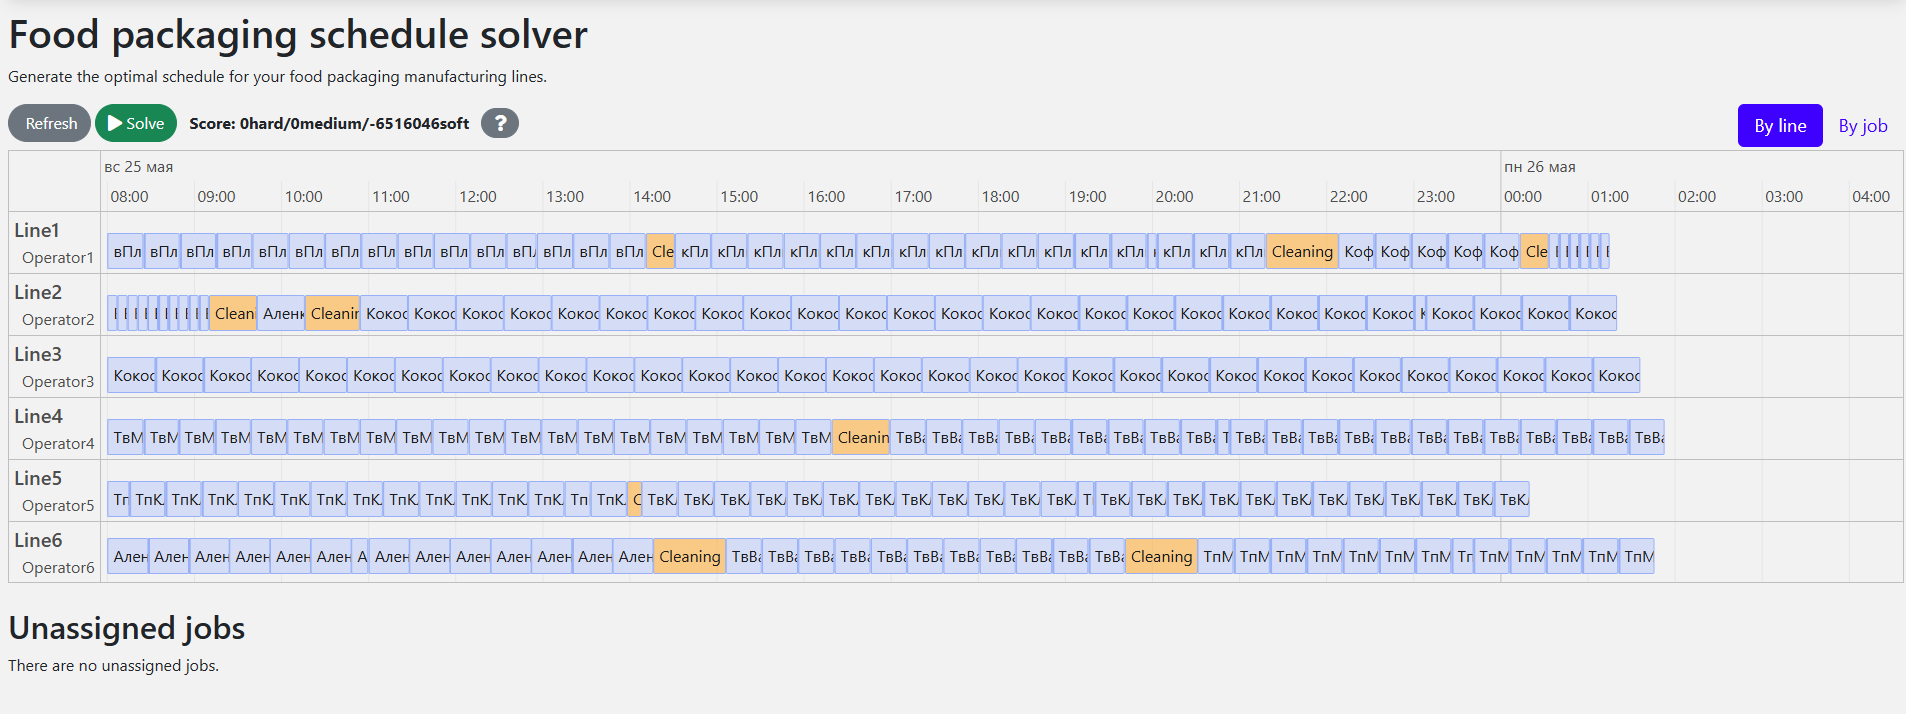
\includegraphics[height = 6 cm, keepaspectratio]{../assets/images/tests/150sec.png}
		\caption{Заявка за 25.05.2025. Время расчета 150 секунд.}
		\label{fig:quarkus_150sec}
\end{figure}

Такая динамика указывает на то, что для качественной минимизации лишней подготовки (мойки) планировщику требуется больше времени. Данное поведение связано с конкуренцией между ограничениями на мягком уровне. В частности, ограничение:

\begin{lstlisting}[caption={Ограничение minimizeCleaningDuration}, label={lst:minimizeCleaningDuration}, basicstyle=\ttfamily\footnotesize, breaklines=true]
protected Constraint minimizeCleaningDuration(ConstraintFactory factory) {
    return factory.forEach(Job.class)
            .filter(job -> job.getStartProductionDateTime() != null)
            .penalizeLong(HardMediumSoftLongScore.ONE_SOFT, job -> 5 * job.getPriority()
                    * Duration.between(job.getStartCleaningDateTime(), job.getStartProductionDateTime()).toMinutes())
            .asConstraint("Minimize cleaning duration");
}
\end{lstlisting}

временно «заглушается» более сильным ограничением \texttt{minimizeAndLoadBalanceMakeSpan}, которое использует квадратичную функцию и имеет преимущество при одинаковом уровне score. Несмотря на это, при длительном времени расчёта Timefold Solver находит компромисс между общим makespan и сокращением длительности санитарной обработки, особенно для заданий с высоким приоритетом.
Данное ограничение начинает влиять на результат только после определённого числа итераций, и его вклад становится ощутимым лишь при расширении временного окна планирования. Таким образом, данный эксперимент демонстрирует, что для достижения качественного и практически применимого расписания требуется не только тщательная формализация ограничений, но и достаточное время для работы планировщика. Оптимальное время порядка 2,5 минут позволяет находить компромисс между жёсткими и мягкими требованиями, что существенно повышает ценность и надёжность разрабатываемой системы планирования.

При анализе эффективности работы планировщика на примере производственной заявки от \textbf{01.06.2025}. Серия запусков с различным лимитом времени на оптимизацию — 90, 120 и 150 секунд — позволила выявить влияние временных ограничений на качество получаемого расписания. На рисунках~\ref{fig:quarkus_90sec_01}, ~\ref{fig:quarkus_120sec_01} и ~\ref{fig:quarkus_150sec_01} представлены скриншоты интерфейса Quarkus с итоговыми результатами планирования.

При расчёте за \textbf{90 секунд} наблюдалась достаточно высокая общая оценка решения с показателями штрафов: \textit{hard} = -18, \textit{medium} = -162, \textit{soft} = -5840340. Наличие ненулевого \textit{hard}-шрафа указывает на нарушение жёстких ограничений, что связано с тем, что часть работ не успевала завершиться до заданного предела в 4:00 утра. Основной узкий участок — линия фасовки продукции типа «Плюш» и «Мишка на Полюсе», ограниченная по возможности выполнения заданий. Дополнительно в расписании наблюдались частые смены одинаковых продуктов на одной линии, что приводило к дополнительным и, по сути, излишним этапам санитарной обработки. Это ухудшало общую эффективность и нарушало логику последовательности.

\begin{figure}[ht]
 \centering
        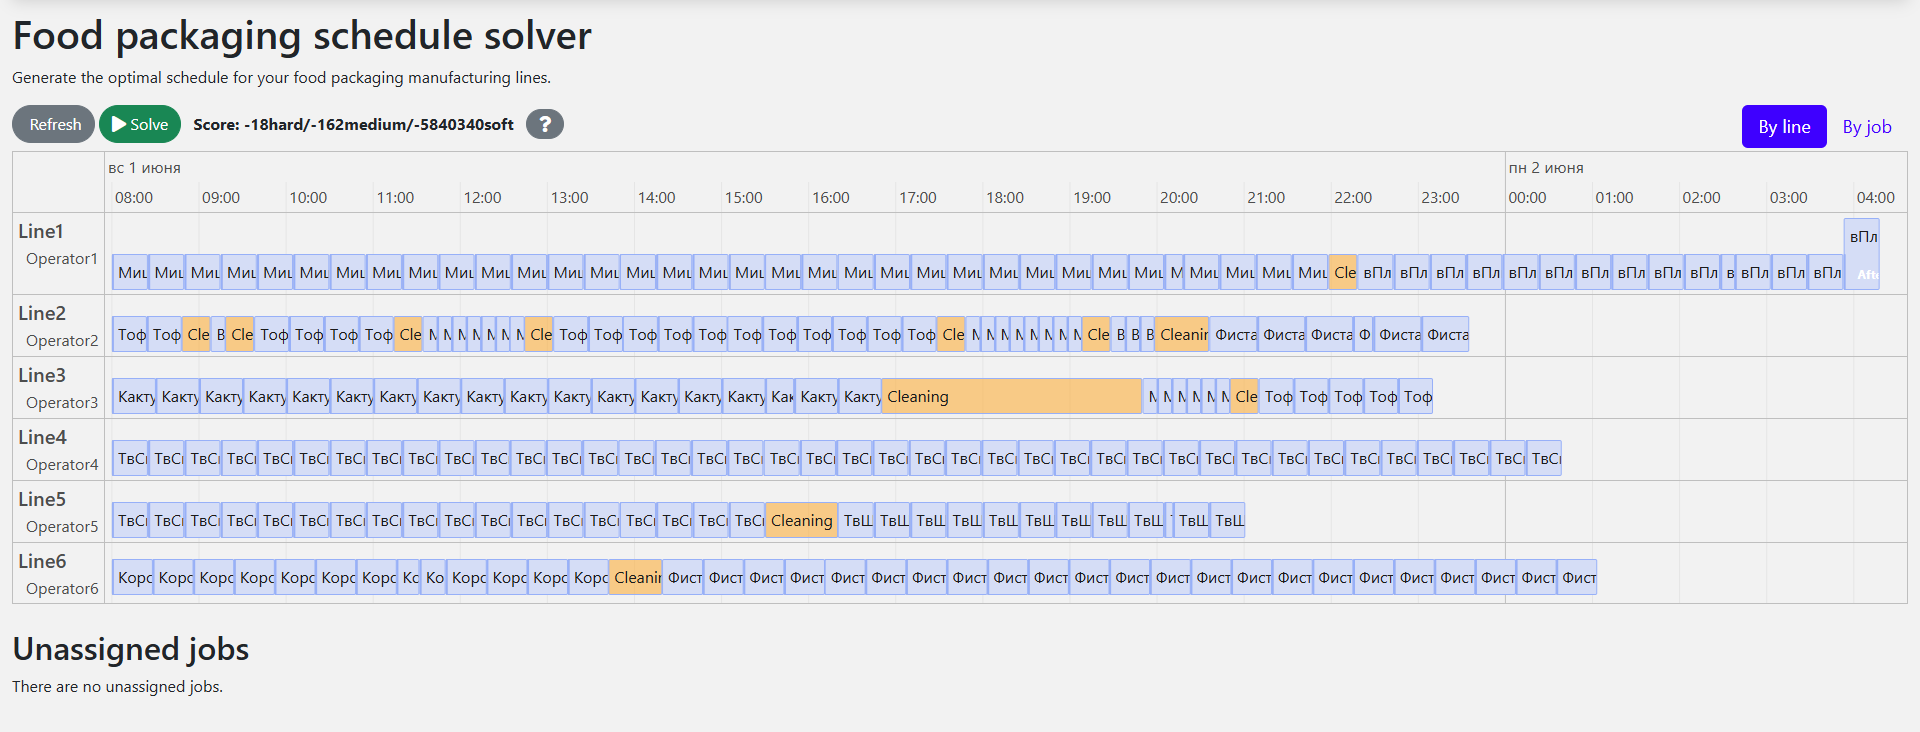
\includegraphics[height = 6 cm, keepaspectratio]{../assets/images/tests/90sec_01.png}
		\caption{Заявка за 01.06.2025. Время расчета 90 секунд.}
		\label{fig:quarkus_90sec_01}
\end{figure}

Увеличение времени решения до \textbf{120 секунд} позволило добиться незначительного снижения \textit{soft}-штрафа до -5660843 при сохранении значений \textit{hard} и \textit{medium} на прежнем уровне. Анализ показал, что благодаря более долгой оптимизации исчезло дублирование заказов в рамках одной линии, однако всё ещё имело место разделение партии одного продукта (например, сырка «Тоффи») между двумя линиями — второй и шестой. Такое разделение приводило к дополнительной мойке, которой можно было бы избежать, если бы фасовка концентрировалась на одной линии. Это свидетельствует о том, что текущая загрузка первой линии не поддаётся перераспределению, а оптимизация более сложных связей и ограничений требует времени.

\begin{figure}[ht]
 \centering
        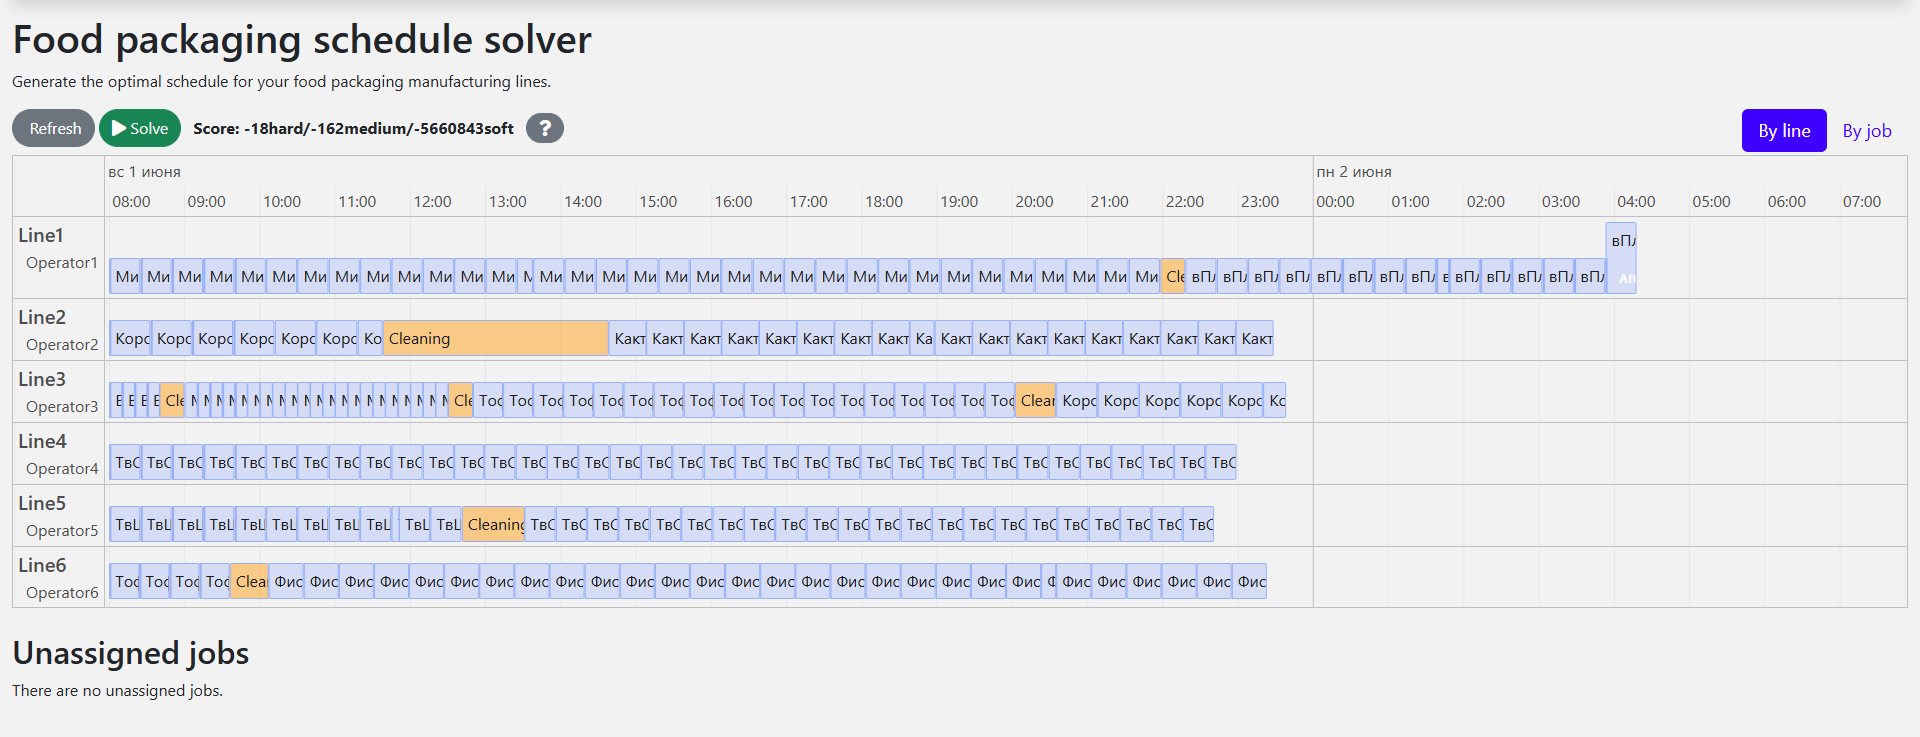
\includegraphics[height = 6 cm, keepaspectratio]{../assets/images/tests/120sec_01.png}
		\caption{Заявка за 01.06.2025. Время расчета 120 секунд.}
		\label{fig:quarkus_120sec_01}
\end{figure}

При максимальном времени планирования — \textbf{150 секунд} — удалось заметно улучшить расписание: \textit{soft}-штраф снизился до -5427668, сохраняя те же значения \textit{hard} и \textit{medium}. Главным достижением стало устранение избыточных моек за счёт устранения нелогичного разделения партий продукции по нескольким линиям, когда их можно было выполнить на одной. Это привело к более компактному и рациональному расписанию, в котором продукция одного типа шла подряд, минимизировалось количество санитарных обработок и учитывались приоритеты заданий.

\begin{figure}[ht]
 \centering
        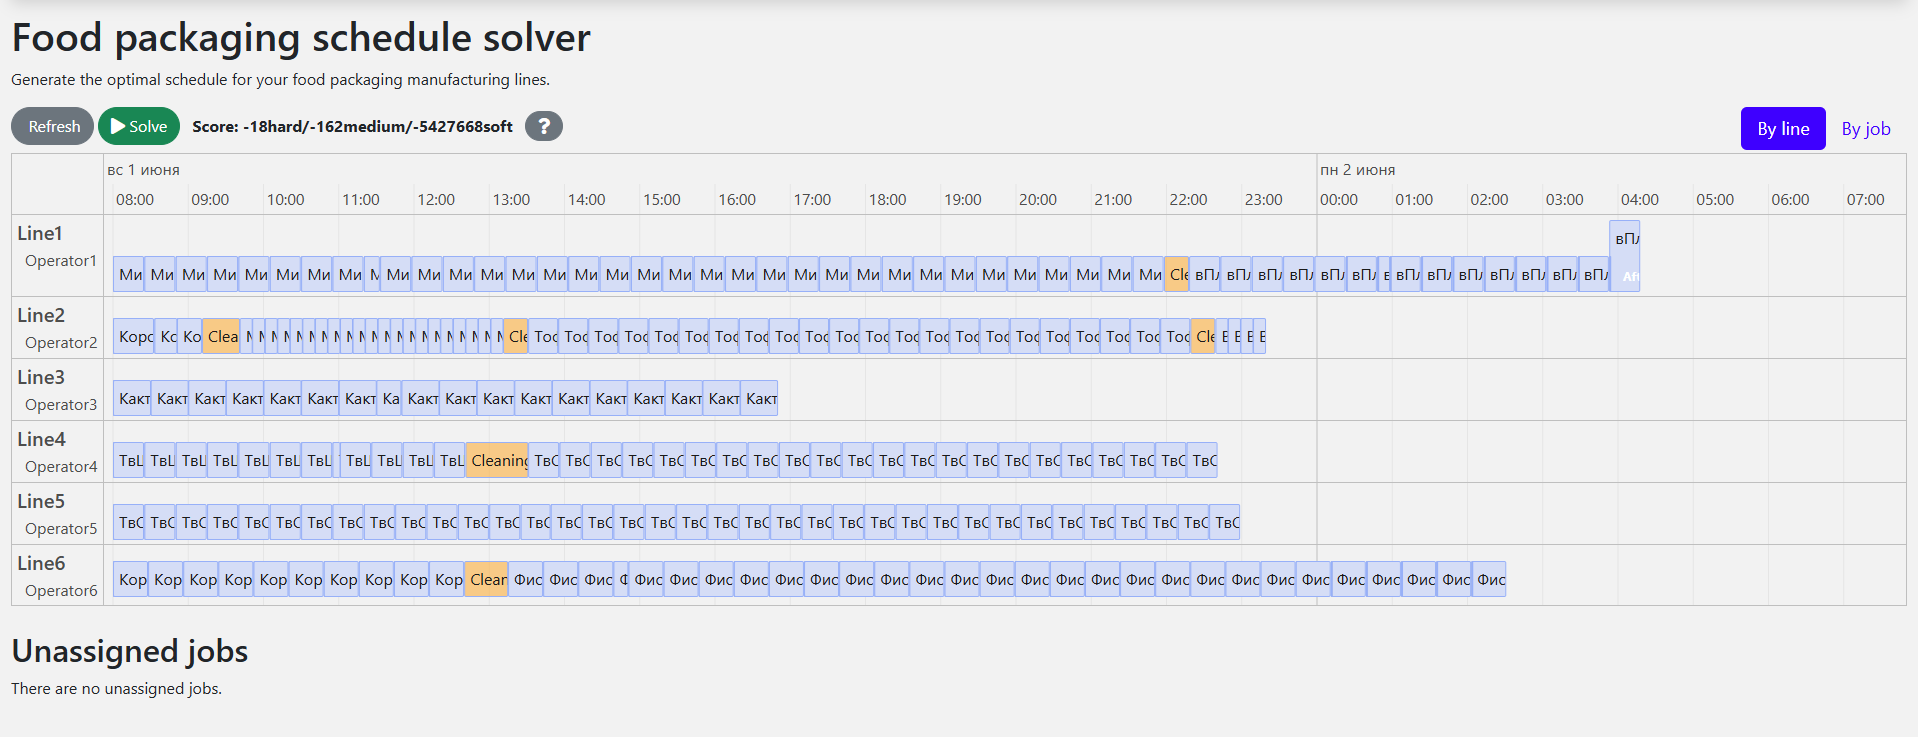
\includegraphics[height = 6 cm, keepaspectratio]{../assets/images/tests/150sec_01.png}
		\caption{Заявка за 01.06.2025. Время расчета 150 секунд.}
		\label{fig:quarkus_150sec_01}
\end{figure}

Динамика изменения качества решений при увеличении времени планирования подчёркивает ключевую роль баланса между временем вычислений и сложностью производственных ограничений. В частности, задача оптимизации санитарных обработок временно «подавляется» более приоритетным ограничением на минимизацию общего времени работы линий (makespan), которое использует квадратичную функцию штрафа и оказывает более сильное влияние на ранних итерациях. Только при увеличении временного окна планирования и глубокой оптимизации проявляется влияние дополнительных ограничений, что видно по улучшению \textit{soft} показателя.

Таким образом, эксперимент подтвердил стабильность и эффективность планировщика при реальных входных данных и времени работы около 2,5 минут.

\section*{Тестирование генерации кода ограничений}

Вторая часть экспериментов была посвящена тестированию нейросетевого модуля генерации Java-кода ограничений, используемых в задаче оптимизации производственного планирования. Целью данной части исследования было определить, насколько эффективно и корректно нейросетевая модель может преобразовать текстовое описание ограничений (на русском языке) в формализованные правила, реализованные с использованием API Constraint Streams библиотеки Timefold Solver. Система тестирования состояла из трёх компонентов, развёрнутых в отдельных Docker-контейнерах: модель машинного перевода с русского на английский язык, модель генерации кода (на основе codegen-2B-multi), а также интерфейс пользователя, реализованный на базе фреймворка Next.js.

\begin{figure}[ht]
    \centering
        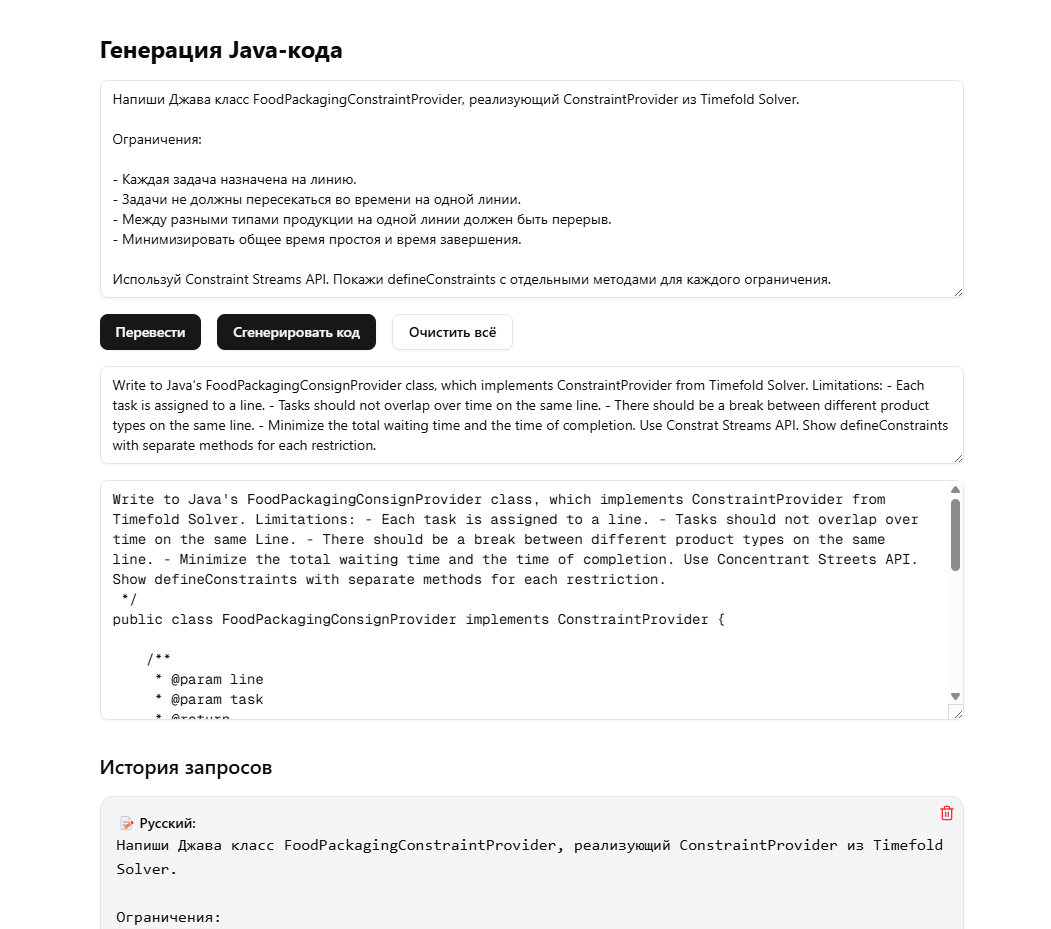
\includegraphics[height = 16 cm, keepaspectratio]{../assets/images/tests/frontend.png}
		\caption{Веб-интерфейс приложения}
		\label{fig:frontend}
\end{figure}


Эксперименты проводились локально с помощью инструмента \texttt{docker-compose}, который обеспечивал скоординированный запуск всех компонентов. Пользователь вводил текстовое описание ограничения в веб-интерфейсе, после чего запрос отправлялся сначала на сервис перевода, а затем — на генератор кода. Далее результат отображался в интерфейсе для последующего анализа.

Одним из показательных примеров стал следующий промпт, описывающий типовые ограничения задачи планирования:

\begin{quote}
{\itshape
Напиши Джава класс \texttt{FoodPackagingConstraintProvider}, реализующий \texttt{ConstraintProvider} из Timefold Solver.

Ограничения:

- Каждая задача назначена на линию.

- Задачи не должны пересекаться во времени на одной линии.

- Между разными типами продукции на одной линии должен быть перерыв.

- Минимизировать общее время простоя и время завершения.

Используй Constraint Streams API. Покажи defineConstraints с отдельными методами для каждого ограничения.
}
\end{quote}

Результат работы модуля перевода оказался неудовлетворительным. В частности, название класса было изменено на \texttt{FoodPackagingConsignProvider}, что является искажением исходного термина. Слово «Constraint» было некорректно переведено как «Consign», что изменило семантику названия. Кроме того, API \texttt{Constraint Streams} было преобразовано в «Constrat Streams», что также негативно повлияло на восприятие запроса моделью генерации кода. Тем не менее, основная структура запроса в переводе сохранилась, включая описание ограничений.

Сама модель генерации кода (codegen-2B-multi) отреагировала на некорректно переведённый запрос следующим образом. В ответе был сгенерирован следующий Java-класс:

\begin{lstlisting}[caption={Ограничение minimizeCleaningDuration}, label={lst:minimizeCleaningDuration}, basicstyle=\ttfamily\footnotesize, breaklines=true]
public class FoodPackagingConsignProvider implements ConstraintProvider {
    /**
     * @param line
     * @param task
     * @return
     */
    @Override
    public List<Constraint> createConstraints(Line line, Task task) {
        List<Constraint> constraints = new ArrayList<>();
        // Get the type of the product
        Type type = task.getProduct().getType();
        // Check if the task is a packing task
        if (task.getProduct().getType() == Type.PACKING) {
            // Create the packing task
            constraints.add(new Constraint("PackagingTask", task));
        }
        return constraints;
    }
}
\end{lstlisting}

Анализ результата показал, что сгенерированный код не соответствует ожидаемой структуре класса \texttt{ConstraintProvider}, принятой в API Timefold Solver. Во-первых, метод \texttt{createConstraints} не является корректным методом интерфейса \texttt{ConstraintProvider} — вместо этого должен использоваться метод \texttt{defineConstraints}, возвращающий массив объектов типа \texttt{Constraint[]}. Во-вторых, генерация кода содержит логические конструкции, не имеющие отношения к описанным ограничениям: используется проверка на тип «PACKING», создаётся искусственный объект \texttt{Constraint} с именем «PackagingTask», но отсутствует работа с временными рамками задач, линиями и приоритетами, необходимыми для корректного решения задачи планирования.

Можно утверждать, что модель не справилась с интерпретацией задачи даже на базовом уровне. Причинами стали, с одной стороны, искажения, внесённые при автоматическом переводе, а с другой — ограниченность архитектуры модели, не способной адекватно соотнести описание бизнес-ограничений с шаблонами Constraint Streams. Также стоит отметить, что структура и формат запроса оказались для модели слишком сложными — в частности, множественные условия и необходимость генерации нескольких методов, каждый из которых реализует отдельное ограничение.

Данный пример показывает важность предварительной подготовки промпта, особенно в условиях многоэтапной генерации, где сначала выполняется перевод, а затем — синтез кода. Даже незначительные искажения в терминах, таких как \texttt{Constraint Streams}, могут привести к полной потере контекста и генерации нерелевантного результата. В последующих экспериментах было принято решение либо использовать англоязычные промпты напрямую, либо вручную контролировать корректность перевода, особенно для критически важных терминов и названий классов. Такой подход позволил добиться более устойчивых результатов и приблизить код к ожидаемой структуре, принятой в Timefold Solver.


\section{Выводы о результатах тестирования}

Результаты проведённого тестирования позволили сделать ряд важных выводов, касающихся как эффективности реализованного планировщика, так и перспектив использования нейросетевых моделей для автоматизации генерации ограничений в системах планирования.

Во-первых, реализованный планировщик на базе Timefold Solver продемонстрировал способность эффективно обрабатывать реальные производственные данные, поступающие из MES-системы. При достаточном времени решения и корректно настроенных параметрах решателя, система надёжно соблюдала как жёсткие, так и мягкие ограничения. В частности, удалось добиться отсутствия пересечений заданий на линиях, соблюдения временных интервалов мойки между различными типами продукции, а также минимизации времени простоя упаковочных линий. Это подтверждает, что Constraint Streams API является мощным инструментом для описания логики производственных процессов.

Во-вторых, эксперименты с нейросетевым модулем генерации Java-кода ограничений показали, что даже компактная языковая модель (в частности, \texttt{codegen-2B-multi}) способна воспроизводить базовые конструкции Constraint Streams. Несмотря на ограниченную точность и частичные ошибки в логике, модель нередко формировала валидные фрагменты кода, включая вызовы \texttt{from()}, \texttt{filter()} и \texttt{penalize()}. Однако при более сложных промптах, требующих точного понимания структуры данных и предметной области, нейросеть допускала логические упрощения и не учитывала особенности API Timefold, такие как приоритеты ограничений, использование \texttt{penalizeLong()} и \texttt{join()}.

Особенно важным оказалось наблюдение, что качество сгенерированного кода напрямую зависит от точности перевода промпта. Так как текст сначала переводился с русского на английский, в некоторых случаях нейросеть-генератор получала искажённый или неестественный вход, что снижало итоговое качество результата. Таким образом, промежуточный этап перевода требует дополнительной фильтрации или редактирования, либо может быть устранён при использовании многоязычных моделей.

Также стоит отметить, что архитектура взаимодействия между компонентами системы, реализованная с использованием Docker-контейнеров и общей сети \texttt{gensolve-net}, показала высокую надёжность и удобство в экспериментах. Все сервисы — веб-интерфейс, модель-переводчик и модель генерации кода — стабильно работали в единой среде, обмениваясь HTTP-запросами. Это подтверждает, что выбранный подход хорошо масштабируется и может быть адаптирован к другим задачам или развернут в облачной инфраструктуре.

В совокупности, полученные результаты подтверждают как жизнеспособность предлагаемой архитектуры, так и потенциал её развития. В перспективе возможно создание обучающей выборки на основе существующих ограничений и fine-tuning нейросетевой модели, способной автоматически генерировать новые ограничения на языке Constraint Streams по текстовому описанию. Это позволит существенно ускорить адаптацию планировщика к новым видам продукции.
